\documentclass[11pt,draft]{article} % use larger type; default would be 10pt
\usepackage{my_packages}

%\usepackage[final]{showlabels} % show labels for referencing

%\usepackage{refcheck} % check for unused references/labels

\title{Coupled Dynamics in the Vicinity of Small Bodies}
\author{Shankar Kulumani}
\date{October 7, 2015}
 % Activate to display a given date or no date (if empty),
         % otherwise the current date is printed 

\begin{document}
\makeatletter
\begin{titlepage}
	\centering
	\LARGE{\@title \par} 
	\vspace{1cm}
	\Large{\@date \par}
	\vfill
	\Large{On my honor, I submit this work in good faith and pledge that I have neither given nor received improper aid in its completion. \par}
	\vspace{1cm}
	\Large{\@author \par}
	\vspace{1cm}
	
\includegraphics{signature}\\
	\vspace{-0.5cm}
	\makebox[2.5in]{\hrulefill}
\end{titlepage}
\makeatother
\section{Motivation}
% why work is important

Small solar system bodies, such as asteroids and comets, are of significant interest for both scientific and economic missions.
These small bodies offer great insight into the early formation of the solar system.
Of particular interest are those near-Earth asteroids (NEA) which inhabit heliocentric orbits in vicinity of the Earth.
These easily accessible bodies provide attractive targets to support space industrialization and mining operations.
NEAs potentially contain many materials useful for propulsion, construction, semiconductors, precious and strategic metals~\cite{ross2001}.
In addition, these NEAs are also of concern for their potential to impact the Earth, and as a result there is a focused effort to mitigate these risks~\cite{wie2008}.
Operating in the vicinity of small planetary bodies is an ongoing and challenging problem for spacecraft missions.

% issues with previous work
% decoupled dynamics
% chaotic enviornment means small perturbations can cause crashes or escape
% fail to exploit dynamic structure (equilibrium points/periodic orbits/invariant manifolds)
% landing methods assume constant gravity
While there has been significant study of interplanetary transfer trajectories, relatively less analysis has been conducted on operations in the vicinity of small bodies.
The dynamic environment of a small body is strongly perturbed and challenging for analysis.
A combination of factors contribute to make operations in the vicinity of small bodies challenging, such as distended body shapes, unknown spin states, relative strength of solar perturbations, and potentially non-gravitational effects in the case of comets~\cite{scheeres2012}.

Previous research near small bodies have considered the translational and rotational dynamics as decoupled~\cite{broschart2005,scheeres1994}.
The spacecraft is assumed to be point masses in orbit about a central body.
However, due to their non-spherical shape there is a direct coupling between the translational and rotational dynamics of a spacecraft.
In addition, as the orbital radius is much larger relative to the body size the impact of this attitude-orbit coupling is much more pronounced than typical Earth based missions. 
Finally, the much weaker gravitational potential of these small bodies also ensures that external disturbances, such as third body effects or solar radiation pressure, are significant.
These perturbations are typically modeled as disturbances rather than directly in the equations of motion. 
However, in the unstable environment of these small bodies even small changes in the state can result in escape or impact trajectories~\cite{scheeres2012}.
As a result, previous work based on a point mass model of the spacecraft are inaccurate and not appropriate for missions in the vicinity of small bodies. 

Since asteroids are not centrobaric bodies, where the point mass assumption is valid, but rather extended bodies there is a much richer dynamic structure.
The full two-body problem governs the combined translation and rotation of two rigid bodies under their mutual gravitational attraction~\cite{fahnestock2006}. 
This mathematical model has many similarities with the three-body problem, specifically there exist equilibrium points as well as periodic orbits about them~\cite{scheeres1994,koon2000}.
Previous missions did not exploit this dynamic structure but rather actively counteracted it through hovering based control or open loop maneuver design~\cite{broschart2005,antreasian2002}.
Unlike the three-body problem, the invariant manifolds of the two-body problem pass very close or intersect with the central body. 
As a result, it is possible to design landing trajectories that exploit the invariant manifolds to reduce the landing costs even further~\cite{herrera2014}.  

%Landing research primarly focused on lunar and Mars descent
%Make constant gravity assumption
%Not typically valid for small bodies with complex gravity potential
%Typically use optimal control methods that are not suitable for on board implementation
%Those asteroid landers have instead used simply preplanned manuevers or vertical control based on laser measurements

% explicitly illustrate how my approach will solve the issues from before

% summary of the proposed contributions and benefits over current approach
In this work, I propose a direct analysis of the coupling between the rotational and translational motion of a spacecraft about a small body. 
The coupling between attitude states and orbital motion will be directly exploited to allow for orbital transfers using only attitude control.
This is in direct contrast to previous work where the orbital dynamics are considered independently of the rotational motion~\cite{kubota2003,antreasian2002}.
In order to effectively harness the effects of small translational forces, the concept of invariant manifolds are extended to the small body environment from their use in the three-body system~\cite{koon2000}. 
Furthermore, these transfers are considered in an under-actuated sense using only attitude control of the spacecraft.
Using the natural dynamics offers the possibility of fuel-free transfers about a small body.

In short, this work will investigate the ability to conduct orbital transfers about small bodies without the use of propellant.
This will utilize the strongly coupled dynamics and investigate under actuated control techniques to offer improved methods for future small body missions.
This capability will enable longer mission life and allow operation in spite of thruster failures or in end of life scenarios.
The use of invariant manifolds combined with the coupled dynamics will allow for innovative methods of orbital transfers and landing on small bodies.

%In addition, more accurate models of the gravitational potential and solar effects are considered in the dynamic model.
%Do not consider coupled dynamics
%Treat rotational motion as decoupled from translational
%
%Ignore dynamic structure that exists in the region of small body
%
%Long integration times with small perturbations not well implemented
%
%Landing dynamics usually assume constant gravity fiel
%
%Direct optimal control formulation - difficult to compute onboard

\section{Literature Review}
\subsection{Small Body Missions}
There have been several recent missions to small bodies in the solar system.
NEAR Shoemaker, Hayabusa, Dawn and the recent Rosetta mission have all operated in proximity of asteroids and comets.
These missions have demonstrated the necessity of accurate dynamic modeling and orbit design capabilities.
In addition, during these missions several have also achieved soft landings onto these bodies. 

In 2001, NEAR Shoemaker became the first spacecraft to make a soft landing on asteroid 433 Eros~\cite{antreasian2002}.
In spite of never being designed for landing, a series of open loop maneuvers were designed to enable a close flyby and a prolonged descent to the surface.
The primary objective was high resolution imagery of the surface with a secondary objective to ensure survival after landing.
A series of maneuvers were planned to achieve a low orbit over the surface followed by a maneuver to kill all lateral velocity relative to the surface. 
These maneuvers did not consider the attitude dynamics of the spacecraft and failed to exploit the dynamic structure of the asteroid environment.

The Hayabusa mission, in contrast to NEAR, never entered into orbit about 25143 Itokawa~\cite{kubota2006}.
The asteroid was small enough that a typical orbit was not possible, rather Hayabusa operated in a so-called ``inertial hovering'' mode.
A series of maneuvers were implemented to ensure that Hayabusa remained inertially fixed relative to the body. 
This placed the vehicle on the Earth-Itokawa line and enabled constant communication with the Earth.
In addition, this position enabled the asteroid to rotate relative to Hayabus enabling near global mapping in support of landing operations.
During the landing sequence, Hayabusa transitioned to a body fixed mode using on-board vision sensors, laser measurements, and a passive tracking marker~\cite{kubota2005}. 
This enabled two touch-and-go landing maneuvers which allowed for the return of surface material to the Earth. 

More recent missions have explored the use of low thrust propulsion.
This has allowed the Dawn mission to visit both asteroid Vesta and Ceres~\cite{rayman2006}.
The computation of of interplanetary trajectories generally uses a point mass model for the spacecraft.
However, in the vicinity of these small bodies the effects of attitude coupling are more pronounced and vital for accurate modeling. 

\subsection{Gravitational Potential}
The classical approach to describing the motion of a objects about a central body has used the point mass approximation~\cite{vallado2001,bate1971}.
Increased sophistication is possible by considering the planetary body as a continuous distribution of matter. 
The gravitational potential of a continuous body on a point mass is most generally defined as 
\begin{equation*}
	\mathcal{U} = G \int_\mathcal{B} \frac{\rho}{\norm{r + \rho}} \, dm \, ,
\end{equation*}
where \( G \) is the universal graviational constant, \( \mathcal{B} \) represents the small body mass distribution, \( r \) is the spacecraft position vector relative to the center of mass of the small body, and \( \rho \) is the position of a differential mass element \( dm \) in the small body fixed frame.
The representation of the gravity potential field is usually expressed using a spherical harmonic representation with a sufficiently large number of terms~\cite{scheeres2012}.
The distributed mass body is modeled in terms of an infinite sum of spherical harmonic coefficients \( C_{lm} \) and \( S_{lm} \).
Away from the body, finite truncations are able to approximate the true potential with good accuracy.
However, when close to the body, or within the Brillouin sphere, this model breaks down and becomes inaccurate or may cause divergence. 
An improvement uses ellipsoidal harmonic coefficients which extends the spherical harmonic representation much closer to the surface of the small body.
However, the ellipsoidal harmonics are difficult to compute and their coefficients are more difficult to estimate.
It is possible to convert the spherical harmonic coefficients directly to their ellipsoidal counterparts which greatly aids in the gravitational modeling process~\cite{dechambre2002}.

Another approach models the gravity field as a constant density polyhedron~\cite{werner1996}.
An advantage of this approach is that small details, such as craters or depressions, can be modeled accurately.
This approach is valid anywhere and accurate for any shape or size of the body. 
The sole source of errors lies in the shape determination and discretization of the body.
However, the constant density assumption can lead to errors. 
In addition, the polyhedral model is complicated to compute for highly detailed shape discretization.

Regardless of the potential model, all are based on the assumption that the spacecraft is accurately represented as a point mass.
This implicit assumption is based on the size of the spacecraft relative to its orbit~\cite{hughes2004}.
The magnitude of the coupling is related to the ratio \( \epsilon = \frac{l}{r} \), where \( l \) is the characteristic spacecraft size and \( r \) is the orbital radius~\cite{sincarsin1983}. 
For Earth mission, this ratio is small, on the order \( \epsilon \approx \num{e-7}\), and the translational dynamics may be considered as decoupled from the orientation.
However, for small bodies this ratio is much larger, on the order of \( \epsilon \approx \num{e-3}\), and the gravitational force is more directly coupled to the orientation.
As a result, it is vital to directly consider the coupled dynamics in mission analysis near small bodies.
%\subsection{Asteroid Soft Landing}
%Landing approaches (constant gravity assumed) - extensions from Lunar/mars missions
%	Summary of Hyabusa and NEAR landing approaches

\section{Proposed Research}
This research is focused on directly using the translation and rotational coupling in the vicinity of small bodies to design orbital transfers.
This model is more realistic and removes the point mass assumption that previous work have utilized. 
Utilizing the structure of the dynamic environment allows for low energy transfers and maneuvers.
Combining this structure with appropriate attitude control will enable orbital transfer maneuvers without the use of propellant.

In order to determine an appropriate attitude control structure a coupled model of the motion of the spacecraft is required.
In addition, dominant perturbing forces such as solar radiation pressure and gravitational effects will also be considered. 
We demonstrate the effect of a rigid body spacecraft using a preliminary numerical simulation about the asteroid 433 Eros.
This highlights the need of incorporating a coupled translational and rotational model for spacecraft about small bodies.

\subsection{Full Two-Body Dynamics}
The dynamics of a spacecraft in the vicinity of a small body are defined using the full two-body problem~\cite{fahnestock2006}.
The spacecraft and small body are modeled as a rigid bodies and are influenced by their mutual gravitational attraction.
This is an extension to the well known two-body problem as it includes the effects of the mass distribution of the bodies.
The configuration space of each body is the special Euclidean group, \( \SE = \R^3 \times \SO \). 
We define a heliocentric inertial reference frame fixed to the Sun. 
A body fixed frame is defined originating at the center of mass of each body of interest and aligned with its principle axes.
The position of each body is defined by \( b_A, b_S \in \R^3 \) which represents the inertial position of the body with respect to the Sun, expressed in the inertial frame. 
The attitude of the each body is defined by \( R_A, R_S \in \SO\) which transforms the representation of a vector from the body-fixed frame to the inertial frame.
The dynamics are defined by
\begin{align*}
	\dot{b} &= R v \, ,\\
	\dot{R} &= R \hat{\Omega} \, ,\\
	m \dot{v} &= m v \times \Omega + \sum F(b, R) \, ,\\
	J \dot{\Omega}  &= J \Omega \times \Omega +  \sum M(b, R) \, ,
\end{align*}
where the translational and rotational velocities are defined in the body fixed frame as \( v , \Omega \in \R^3 \), respectively.

This general form of the coupled dynamics allows for a variety of forces to be modeled.
The external forces and moments, \( F, M \in \R^3 \) respectively, are expressed in the body fixed frame and represent the forces due to the gravity and solar effects.
We assume the small body, or asteroid, is only under the influence of a gravitational force and moment caused by the Sun.
This means that the motion of the spacecraft does not affect the motion of the asteroid. 
However, the motion of the spacecraft is influenced by both the asteroid and the Sun.
We can model the effect of the asteroid using any of the previously mentioned gravitational potential models. 
However, there is a tradeoff between accuracy and ease of implementation as well as the opportunity for analytical insight. 
%In addition, the spacecraft experiences a moment caused by solar radiation pressure.
As result, its dynamics are coupled due to the position and attitude dependent forces and moments.
\subsection{Gravitational Potential}
The gravitational potential of the asteroid may be expanded using a spherical harmonic expansion as
\begin{align*}
	\mathcal{U} &= \frac{\mu}{r} \sum_{n=0}^\infty \sum_{m=0}^\infty \parenth{\frac{R}{r}}^nP_{n,m}(\sin \phi) \braces{ C_{nm} \cos(m \lambda) + S_{nm} \sin(m \lambda)} \, , \\
	P_{n,m}(\sin \phi) &= \frac{1}{2^n n !} \parenth{1 - \sin^2 \phi}^{m/2} \frac{d^{n+m}}{d \parenth{\sin \phi}^{n+m}} \parenth{\sin^2 \phi -1}^n \, ,
\end{align*}
where \( \mu \) is the gravitational parameter of the body, \( R \) is the radius of the circumscribing sphere and \( \phi, \lambda \) are the geodetic latitude and longitude respectively~\cite{vallado2001}.

In order to allow for analytical insight, a constant density triaxial ellipsoidal model is assumed for the preliminary analysis. 
The asteroid is also assumed to rotate about the axis of maximum moment of inertia at a constant rate.
This allows for the major shape perturbations of the asteroid to be expressed in closed form~\cite{scheeres1994}.
In addition, the triaxial ellipsoid model is popular as it incorporates the effects of the most significant shape characteristics and can be specified based on optical measurements alone.
This allows one to define a potential model of an asteroid prior to arrival and detailed measurements. 
Even with the addition of increased terms or a polyhedral potential model the dynamic structure is not radically altered. 
This allows for analytical insight prior to the determination of an accurate potential model.

This type of model allows for dynamic insight into the motion about the asteroid.
A Lagrangian is formed as the difference between the kinetic and potential energies, \( L(q, \dot{q}, t) =T - V \).
If it is possible to transform the Lagrangian into a reference frame where it is time invariant, one may define a constant or integral of motion~\cite{greenwood1988}.
The Jacobi integral, \( h = \sum_{i=1}^n \deriv{L}{\dot{q}_i} \dot{q}_i - L(q,\dot{q}) \), is an energy-like constant useful for analysis.
The existence of this integral allows the use of zero-velocity surfaces to be defined and govern the stability.
In addition, this implies that equilibrium points can exist as well as families of periodic orbits in these systems~\cite{scheeres2012}.
 
This structure is similar to that of the three-body problem and allows for a variety of stable and unstable manifolds~\cite{hu2002}.
In addition, analysis of the dynamic environment allows for energy free transfers about the asteroid and can be extended to landing~\cite{herrera2014}.
Previous work has treated the spacecraft as a point mass rather than an extended rigid body.
This ignores the significant effects of attitude dependent forces and moments on the vehicle and the resulting trajectory. 
We avoid this by directly considering a coupled model of the spacecraft.
Using attitude control, it is desired to design transfers that allow traversal of the phase space without the use on-board propulsion.

%\subsection{Solar Perturbations}
%Discuss order of perturbations are the same for solar and gravity terms
%
%Use a flat plate model to approximate force and moment impart by solar radiation pressure. 
%
%More complicated models incorporate surface properties of the body (reflectivity, absorption, specular vs diffuse)

\section{Preliminary Results}
\begin{figure}
	\centering 
	\begin{subfigure}[htbp]{0.3\textwidth} 
		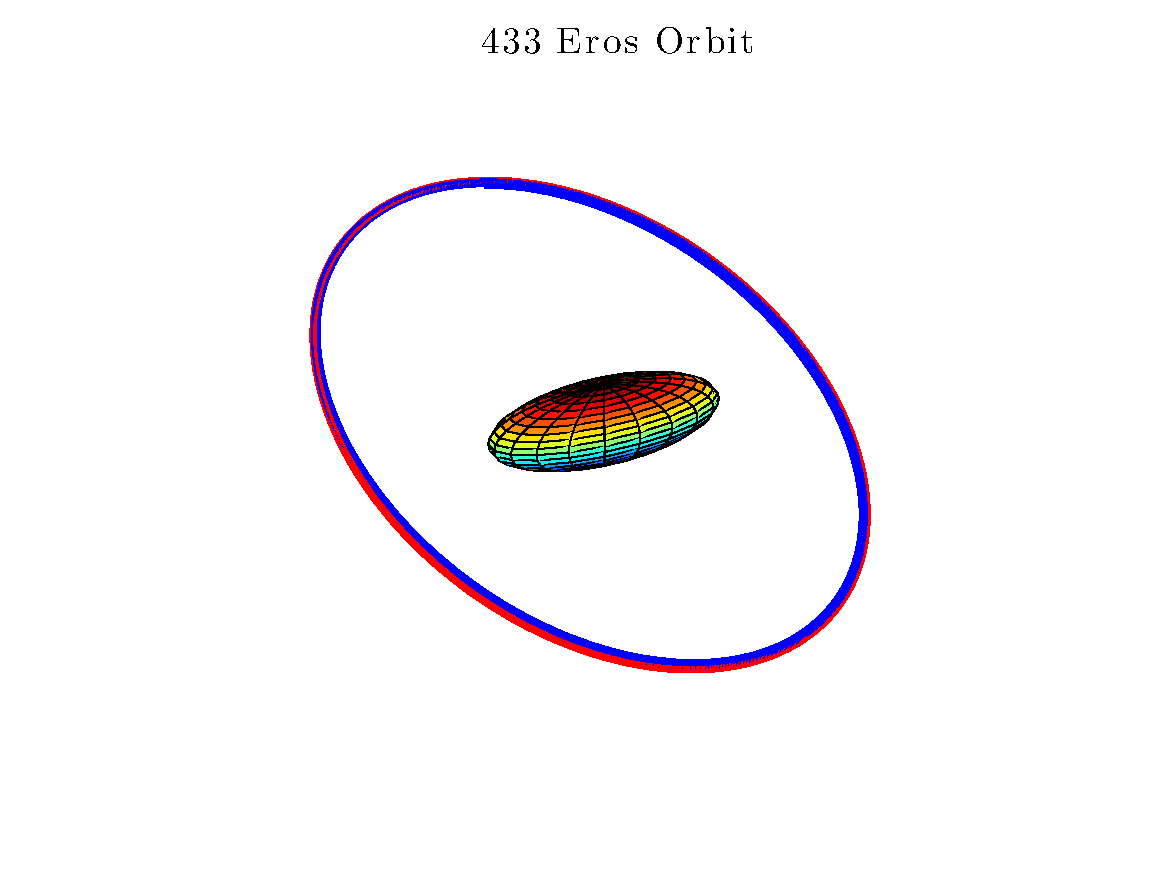
\includegraphics[width=\textwidth]{10orbits} 
		\caption{\num{10} Orbits} \label{fig:10orbits} 
	\end{subfigure}~ %add desired spacing between images, e. g. ~, \quad, \qquad, \hfill etc. %(or a blank line to force the subfigure onto a new line) 
	\begin{subfigure}[htbp]{0.3\textwidth} 
		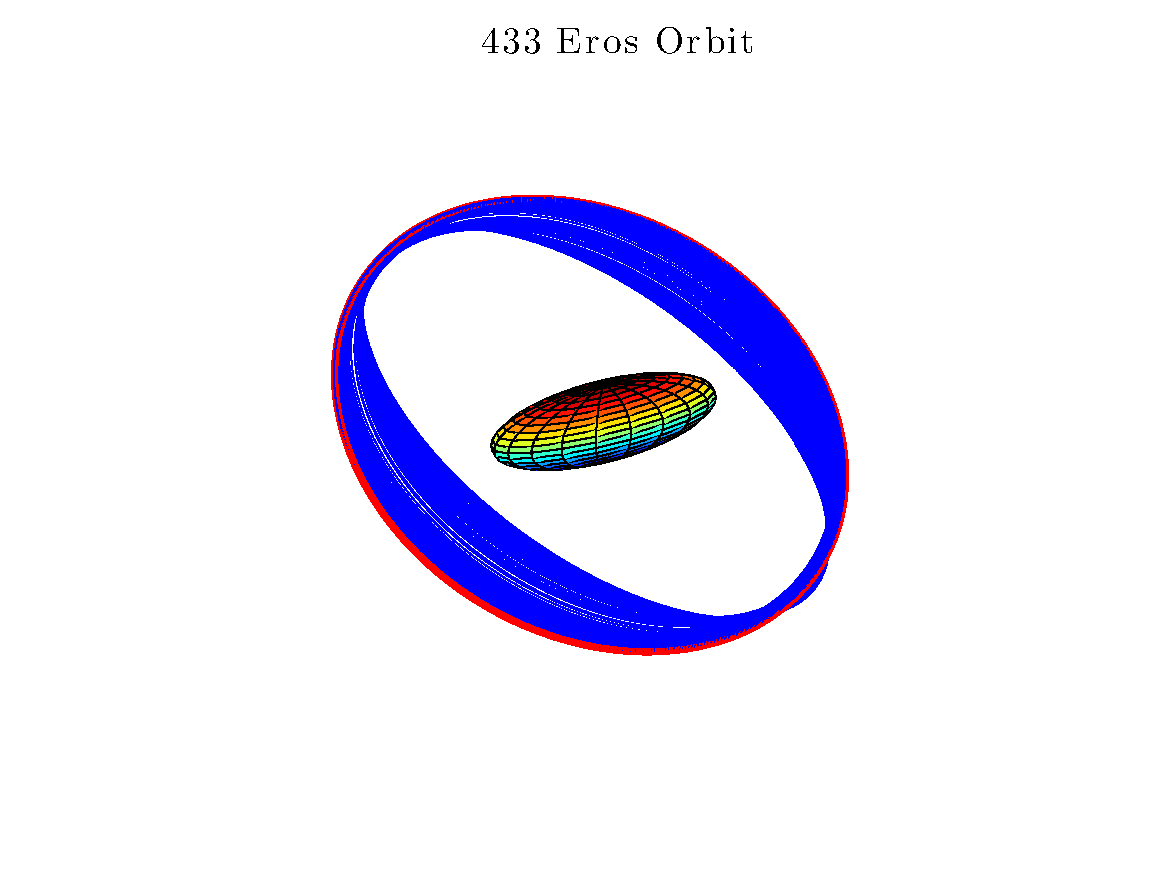
\includegraphics[width=\textwidth]{50orbits} 
		\caption{\num{50} Orbits} \label{fig:50orbits} 
	\end{subfigure} ~ %add desired spacing between images, e. g. ~, \quad, \qquad, \hfill etc. %(or a blank line to force the subfigure onto a new line) 
	\begin{subfigure}[htbp]{0.3\textwidth} 
		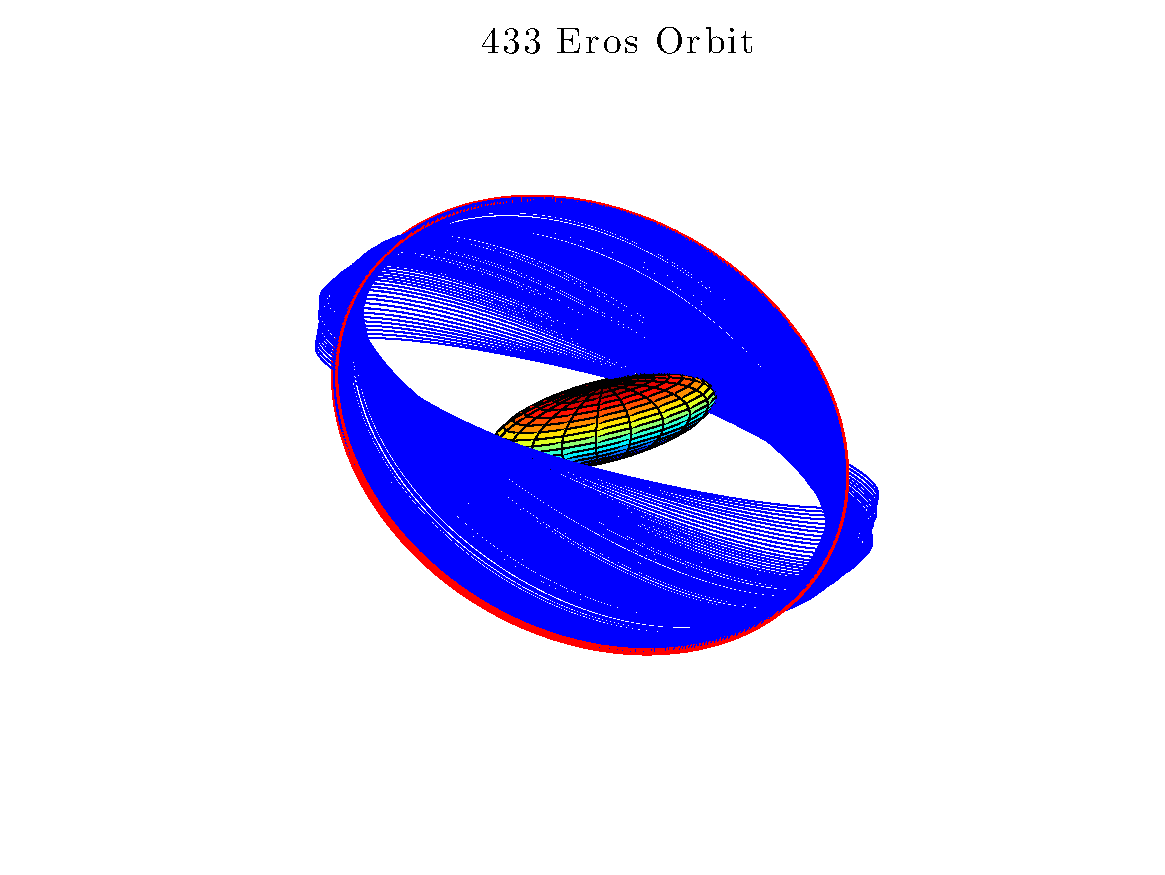
\includegraphics[width=\textwidth]{100orbits} 
		\caption{\num{100} Orbits} \label{fig:100orbits} 
	\end{subfigure} 
	\caption{Rigid Body Perturbation}
	\label{fig:orbits} 
\end{figure}

A preliminary simulation is conducted to demonstrate the effects of coupled rotational and translational dynamics of a spacecraft near an asteroid.
We represent asteroid 433 Eros as a triaxial ellipsoid and use the second degree and order gravitational potential terms~\cite{hu2008,scheeres2003}.
This is the simplest non-trivial potential model that captures the significant contributions of a continuous mass distribution~\cite{scheeres2012a}.
The gravitational potential of Eros is defined as
\begin{align*}
	\mathcal{U} = \frac{\mu_A}{\norm{r}}-\frac{\mu_A C_{20} \parenth{x^2 + y^2 - 2 z^2}}{2 \norm{r}^5} + \frac{3 \mu_A C_{22} \parenth{x^2 - y^2}}{\norm{r}^5}\, ,
\end{align*}
where \( r = \begin{bmatrix} x & y & z \end{bmatrix} \) is the position of the spacecraft relative to the asteroid, represented in the asteroid fixed frame.
The gravitational force and moment due to the asteroid on the spacecraft are calculated using this form of potential function.
In spite of this relatively simple model, \Cref{fig:orbits} shows the effect of the orbit-attitude coupling on the motion of a spacecraft.
Over time the effect of the attitude dependent gravitational force greatly perturbs the trajectory.
This effect is magnified due to the distended shape of 433 Eros.
Rather than having a tumbling spacecraft, an attitude control scheme will be generated to control the translational forces on the spacecraft. 
This will be used to maintain desired orbits as well as conduct transfers using invariant manifolds.

In the vicinity of small bodies there is a strong coupling between translational and rotational motion.
These preliminary clearly demonstrate the effect of an attitude dependent on the motion of a spacecraft. 
Neglecting these effects is both inaccurate and inefficient. 
The goal of this work is the design of attitude control systems that harness the strongly perturbed dynamics near small bodies to enable fuel free transfers and landings.

%Insight into dynamics by allowing analytical results
%Possible to obtain this model solely from ground based observations
%Allows for insight into structure that will also exist once more accurate models are implemented.
%Second order and degree gravitational field 
%
%Show effect of rigid body spacecraft vs point mass spacecraft
%Summarize benefits of this approach over previous work

\bibliographystyle{unsrt}
\bibliography{library}

\end{document}
